\documentclass{article}
\usepackage{tikz}

\pagenumbering{gobble}
\begin{document}

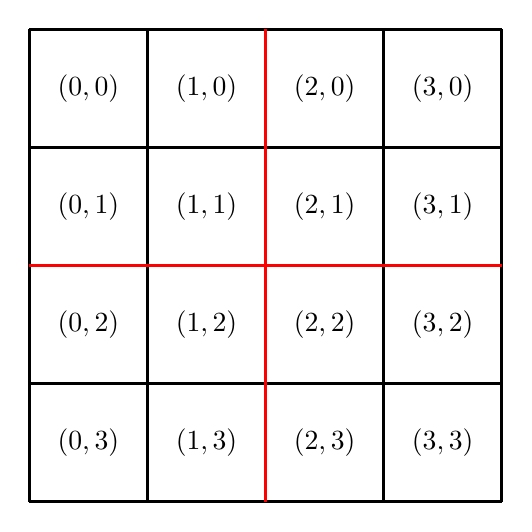
\begin{tikzpicture}[scale=1.5]
    \foreach \i in {0,...,4} {
        \draw [very thick,black] (\i,0) -- (\i,4);
    }
    \foreach \i in {0,...,4} {
        \draw [very thick,black] (0,\i) -- (4,\i);
    }
    \draw [very thick,red] (2,0) -- (2,4);
    \draw [very thick,red] (0,2) -- (4,2);
    \foreach \i in {0,...,3} {
       \foreach \j in {0,...,3} {
           \pgfmathparse{int(Mod(\i,4))}
           \let\ii\pgfmathresult
           \pgfmathparse{int(Mod(\j,4))}
           \let\jj\pgfmathresult
           \node at (\i+0.5,3-\j+0.5) {$(\ii, \jj)$};
       }
    }
\end{tikzpicture}

\vspace{10mm}

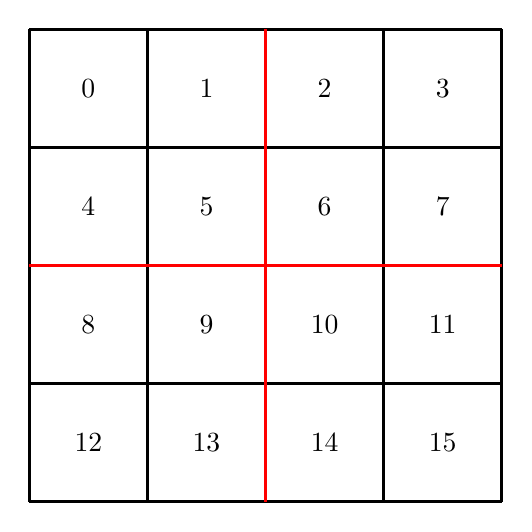
\begin{tikzpicture}[scale=1.5]
    \foreach \i in {0,...,4} {
        \draw [very thick,black] (\i,0) -- (\i,4);
    }
    \foreach \i in {0,...,4} {
        \draw [very thick,black] (0,\i) -- (4,\i);
    }
    \draw [very thick,red] (2,0) -- (2,4);
    \draw [very thick,red] (0,2) -- (4,2);
    \foreach \i in {0,...,3} {
       \foreach \j in {0,...,3} {
           \pgfmathparse{int(\j * 4 + \i)}
           \let\ii\pgfmathresult
           %\pgfmathparse{int(Mod(\j,4))}
           %\let\jj\pgfmathresult
           \node at (\i+0.5,3-\j+0.5) {$\ii$};
       }
    }
\end{tikzpicture}

\vspace{10mm}

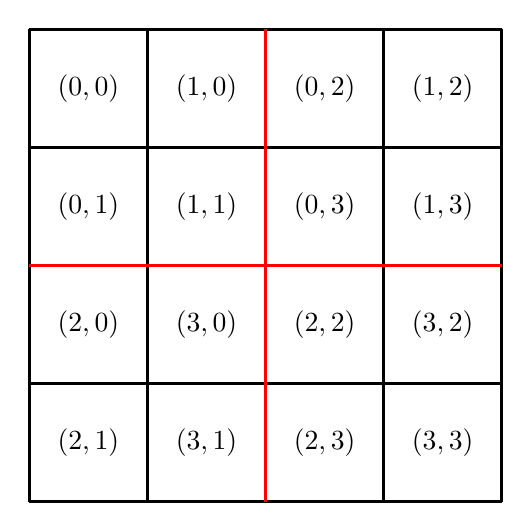
\begin{tikzpicture}[scale=1.5]
    \foreach \i in {0,...,4} {
        \draw [very thick,black] (\i,0) -- (\i,4);
    }
    \foreach \i in {0,...,4} {
        \draw [very thick,black] (0,\i) -- (4,\i);
    }
    \draw [very thick,red] (2,0) -- (2,4);
    \draw [very thick,red] (0,2) -- (4,2);
    \foreach \i in {0,...,3} {
       \foreach \j in {0,...,3} {
           \pgfmathparse{int(Mod(\i,2)+int(\j / 2)*2}
           \let\ii\pgfmathresult
          \pgfmathparse{int(Mod(\j,2)+int(\i / 2)*2}
           \let\jj\pgfmathresult
           \node at (\i+0.5,3-\j+0.5) {$(\ii, \jj)$};
       }
    }
\end{tikzpicture}

\vspace{10mm}

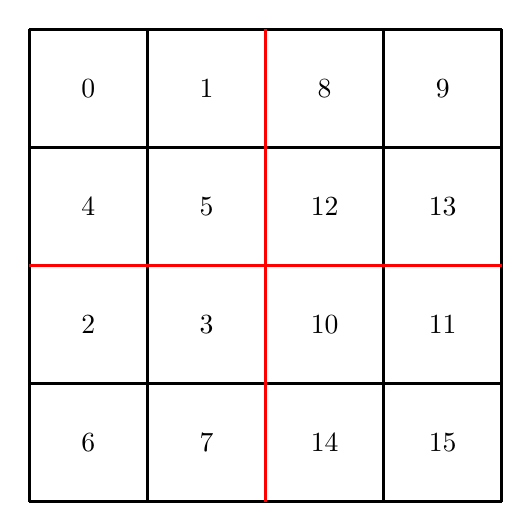
\begin{tikzpicture}[scale=1.5]
    \foreach \i in {0,...,4} {
        \draw [very thick,black] (\i,0) -- (\i,4);
    }
    \foreach \i in {0,...,4} {
        \draw [very thick,black] (0,\i) -- (4,\i);
    }
    \draw [very thick,red] (2,0) -- (2,4);
    \draw [very thick,red] (0,2) -- (4,2);
    \foreach \i in {0,...,3} {
       \foreach \j in {0,...,3} {
           \pgfmathparse{int(Mod(\i,2)+int(\j / 2)*2}
           \let\ii\pgfmathresult
          \pgfmathparse{int(Mod(\j,2)+int(\i / 2)*2}
           \let\jj\pgfmathresult
           \pgfmathparse{int(\jj * 4 + \ii)}
           \let\kk\pgfmathresult
           \node at (\i+0.5,3-\j+0.5) {$\kk$};
       }
    }
\end{tikzpicture}

\vspace{10mm}

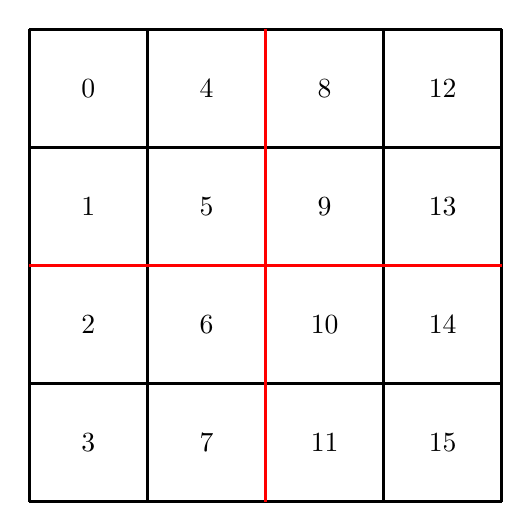
\begin{tikzpicture}[scale=1.5]
    \foreach \i in {0,...,4} {
        \draw [very thick,black] (\i,0) -- (\i,4);
    }
    \foreach \i in {0,...,4} {
        \draw [very thick,black] (0,\i) -- (4,\i);
    }
    \draw [very thick,red] (2,0) -- (2,4);
    \draw [very thick,red] (0,2) -- (4,2);
    \foreach \i in {0,...,3} {
       \foreach \j in {0,...,3} {
           \pgfmathparse{int(\j * 4 + \i)}
           \let\ii\pgfmathresult
           %\pgfmathparse{int(Mod(\j,4))}
           %\let\jj\pgfmathresult
           \node at (\j+0.5,3-\i+0.5) {$\ii$};
       }
    }
\end{tikzpicture}

\end{document}
